\documentclass[]{article}
\usepackage{amsmath}
\usepackage{amssymb}
\usepackage{amsthm}
\usepackage[T1]{fontenc}
\usepackage{indentfirst}
\usepackage{listings}
\usepackage{tikz}
\usepackage{tikz-qtree}
\usepackage{tipa}
\usetikzlibrary{arrows,automata}
\begin{document}

\title{COMS W3261 \\ Computer Science Theory \\ Chapter 8 Notes}
\author{Alexander Roth}
\date{2014--10--10}
\maketitle
\theoremstyle{definition}
\newtheorem{thm}{Theorem}
\section*{Introduction to Turing Machines}
Until now, we have been interested primarily in simple classes of languages 
and the ways that they can be used for relatively constrained problems, such 
as analyzing protocols, searching text, or parsing programs. Now, we shall 
start looking at the question of what languages can be defined by any 
computational device whatsoever. This question is tantamount to the question 
of what computers can do, since recognizing the strings in a language is a 
formal way of expressing any problem, and solving a problem is a reasonable 
surrogate for what it is that computers do. \\
\indent We begin with an informal argument to show that there are specific 
problems that we cannot solve using a computer. These problems are called 
``undecidable.'' We then introduce a venerable formalism for computers, 
called the Turing machine. The Turing machine has long been recognized as an 
accurate model for what any physical computing device is capable of doing.

\section*{Problems That Computers Cannot Solve}
The purpose of this section is to provide an informal, C-programming-based
introduction to the proof of a specific problem that computers cannot solve. 
The particular problem we discuss is whether the first thing a C program 
prints is \texttt{hello, world}. Although we might imagine that simulations 
of the program would allow us to tell what the program does, we must in 
reality contend with programs that take an unimaginably long time before 
making any output at all. This problem -- not knowing when, if ever, 
something will occur -- is the ultimate cause of our inability to tell what a 
program does. However, proving formally that there is no program to do a 
stated task is quite tricky, and we need to develop some formal mechanics.

\subsection*{Programs that Pring ``Hello, World''}
Below is the first C program met by students who read Kernighan and 
Ritchie's classic book. It is rather easy to discover that this program 
prints \texttt{hello, world} and terminates.

\lstinputlisting[language=C]{../hello_world.c}

However, there are other programs that also print \texttt{hello, world}; 
yet the fact that they do so is far from obvious

\lstinputlisting[language=C]{../obfuscated_hello_world.c}

This program takes as input $n$, and looks for positive integer solutions 
to the equation $x^n + y^n = z^n$ If it finds one, it prints 
\texttt{hello, world}

To understand what this program does, first observer that \texttt{exp} is 
an auxiliary function to compute exponentials. The main program needs to 
search through triples $(x,y,z)$ in an order such that we are sure we get 
to every triple of positive integers eventually. To organize the search 
properly, we use a fourth variable, \texttt{total}, that starts at 3 and, 
in the while-loop, is increased one unit at a time, eventually reaching any 
finite integer. Inside the while-loop, we divide \texttt{total} into three 
positive integers $x$, $y$, and $z$, by first allowing $x$ to range from 1 
to \texttt{total-2}, and within that for-loop allowing $y$ to range from 1 
up to one less than what $x$ has not already taken from \texttt{total}. 
What remains, which must be between 1 and \texttt{total-2} is given to $z$.

In the innermost loop, the triple $(x,y,z)$ is texted to see if
$x^n + y^n = z^n$. If so, the program prints \texttt{hello, world}.

If the value of $n$ that the program reads is 2, then it will eventually 
find combinations of integers such as \texttt{total} = 12, 
$x = 3$, $y = 4$,
and $z = 5$, for which $x^n + y^n = z^n$. Thus, for input 2, the program 
will \emph{does} print \texttt{hello, world}. However, for any integer 
$n > 2$, the program will never find a triple of positive integer to 
satisfy $x^n + y^n = z^n$.

Let us define the \emph{hello-world problem} to be: determine whether a 
given C program, with a given input, prints \texttt{hello, world} as the 
first 12 characters that it prints.

\subsubsection*{Why Undecidable Problems Must Exist}
Recall that a ``problem'' is really membership of a string in a 
language. The number of different languages over any alphabet of more 
than one symbol is not countable. That is, there is no way to assign 
integers to the languages such that every language has an integer, and 
every integer is assigned to one language.

On the other hand programs, being finite strings over a finite alphabet
\emph{are} countable. That is, we can order them by length, and for
programs of the same length, order them lexicographically. Thus, we can
speak of the first program, the second program, and in general, the 
$i$th program for any integer $i$.

As a result, we know there are infinitely fewer program than there are
problems. If we picked a language at random, almost certainly it would 
be an undecidable problem. The only reason that most problems 
\emph{appear} to be decidable is that we rarely are interested in 
random problems. Rather, we tend to look at fairly simple,, well-
structured problems, and indeed these are often decidable. However, 
even among the problems we are interested in and can state clearly and 
succinctly, we find many that are undecidable; the hello-world problem 
is a case in point.

\subsection*{The Hypothetical ``Hello, World'' Tester}
The proof of impossibility of making the hello-world test is a proof by
contradiction. That is, we assume there is a program, call it $H$, that 
takes as input a program $P$ and an input $I$, and tells whether $P$ with 
input $I$ prints \texttt{hello, world}. In particular, the only output $H$ 
makes is either to print the three characters \texttt{yes} or to print the 
two characters \texttt{no}. It always does one or the other.

If a problem has an algorithm like $H$, that always tells correctly an 
instance of the problem has answer ``yes'' or ``no,'' then the problem is
said to be ``decidable.'' Otherwise, the problem is ``undecidable.''

In order to prove that statement by contradiction, we are going to make
several changes to $H$, eventually constructing a related program called
$H_2$ that we does not exist. Since the changes to $H$ are simple
transformations that can be done to any C program, the only questionable
statement is the existence of $H$, so it is that assumption we have
contradicted.

To simplify our discussion, we shall make a few assumptions about C 
programs. These assumptions make $H$'s job easier so if we can show a
``hello-world tester'' for these restricted programs does not exist, then
surely there is no such tester that could work for a broader class of 
programs. Our assumptions are:
\begin{enumerate}
\item All output is character-based, e.g., we are not using a graphics
package or any other facility to make output that is not in the form of
characters.
\item All character-based output is performed using \texttt{printf},
rather than \texttt{putchar()} or another character-based output 
function. 
\end{enumerate}

We now assume that the program $H$ exists. Our first modification is to 
change the output \texttt{no}, which is the response that $H$ makes when
its input program $P$ does not print \texttt{hello, world} as its first 
output in response to input $I$. As soon as $H$ prints ``n'', we know it 
will eventually follow with ``o''. Thus, we can modify any \texttt{printf}
statement in $H$ that prints ``n'' to instead print \texttt{hello, world}.
Another \texttt{printf} statement that prints ``o'' but not the ``n'' is
omitted. As a result, the new program, which we call $H_1$, behaves like 
$H$, except it prints \texttt{hello, world} exactly when $H$ would print
\texttt{no}.

Our next transformation on the program is a bit trickier; it is essentially
the insight that allowed Alan Turing to prove his undecidability result 
about Turing machines. Since we are really interested in programs that take
other programs as input and tell something about them, we shall restring
$H_1$ so it:
\begin{enumerate}
\item[a)] Takes only input $P$, not $P$ and $I$.
\item[b)] Asks what $P$ would do if its input were its own code, i.e.,
what would $H_1$ do on inputs $P$ as program and $P$ as input $I$ as 
well?
\end{enumerate}

The modifications we must perform on $H_1$ to produce the program $H_2$ are
as follows:
\begin{enumerate}
\item $H_2$ first reads the entire input $P$ and stores it in an array
$A$, which it ``malloc's'' for the purpose.
\item $H_2$ then simulates $H_1$, but whenever $H_1$ would read input 
from $P$ or $I$. $H_2$ reads from the stored copy in $A$. To keep track 
of how much of $P$ and $I$ $H_1$ has read, $H_2$ can maintain two
cursors that mark positions in $A$.
\end{enumerate}

We are now ready to prove $H_2$ cannot exist. Thus, $H_1$ does not exist,
and likewise, $H$ does not exist. The heart of the argument is to envision
what $H_2$ does when given itself as input. Recall that $H_2$, given any
program $P$ as input, makes output \texttt{yes} if $P$ prints 
\texttt{hello, world} as its first output.

Suppose that the $H_2$ makes the output \texttt{yes}. Then $H_2$ that is 
receiving as input $H_2$ is saying about its input $H_2$ that $H_2$, given
itself as input, prints \texttt{hello, world} as its first output. But we 
just supposed that the first output $H_2$ makes in this situation is 
\texttt{yes} rather than \texttt{hello, world}.

Thus it appears that the output of the machine is \texttt{hello, world},
since it must be one or the other. But if $H_2$, given itself as input,
prints \texttt{hello, world} first, then the output of the machine must be
\texttt{yes}. Whichever output we suppose $H_2$ makes, we can argue that it
makes the other output.

This situation is paradoxical, and we conclude that $H_2$ cannot exist. As 
a result, we have contradicted the assumption that $H$ exists.

\subsection*{Reducing One Problem to Another}
A problem that cannot be solved by computer is called \emph{undecidable}.
Suppose we want to determine whether or not some other problem is solvable
by a computer. We can try to write a program to solve it, but if we cannot
figure out how to do so, then we might try a proof that there is no such
program.

Once we have one problem that we know is undecidable, we no longer have to
prove existence of a paradoxical situation. It is sufficient to show that 
if we could solve the new problem, then we could use that solution to solve 
a problem we already know is undecidable. This technique is called the
\emph{reduction} of $P_1$ to $P_2$.

Suppose that we know problem $P_1$ is undecidable, and $P_2$ is a new
problem that we would like to prove is undecidable as well. We suppose that
there is a program that prints \texttt{yes} or \texttt{no}, depending on 
whether its input instance of problem $P_2$ is or is not in the language of 
that problem.

In order to make a proof that problem $P_2$ is undecidable, we have to
invent a construction that converts instances of $P_1$ to instances of 
$P_2$ that have the same answer. That is, any string in the language $P_1$ 
is converted to some string in the language $P_2$, and any string over the
alphabet of $P_1$ that is \emph{not} in the language $P_1$ is converted to 
a string that is not in the language $P_2$. Once we have this construction, 
we can solve $P_1$ as follows:
\begin{enumerate}
\item Given an instance of $P_1$, that is, given a string $w$ that may 
or may not be in the language $P_1$, apply the construction algorithm 
to produce a string $x$.
\item Test whether $x$ is in $P_2$, and give the same answer about $w$
and $P_1$.
\end{enumerate}

If $w$ is in $P_1$, then $x$ is in $P_2$, so this algorithm says 
\texttt{yes}. If $w$ is not in $P_1$, then $x$ is not in $P_2$, and the 
algorithm says \texttt{no}. Since we assumed that no algorithm to decide
membership of a string in $P_1$ exists, we have a proof by contradiction 
that the hypothesized decision algorithm for $P_2$ does not exist; i.e., 
$P_2$ is undecidable.

\section*{The Turing Machine}
The purpose of the theory of undecidable problems is not only to establish 
the existence of such problems but to provide guidance to programmers about 
what they might or might not be able to accomplish through programming. These 
problems, called ``intractable problems,'' tend to present greater difficulty 
to the programmer and the system designer that do the undecidable problems. 
The reason is that, while undecidable problems are usually quite obviously 
so,and their solutions are rarely attempted in practice, the intractable 
problems are faced every day. Moreover, they often yield to small 
modifications in the requirements or to heuristic solutions. Thus, the 
designer is faced quite frequently with having to decide whether or not a 
problem is in the intractable class, and what to do about it, if so.

We need tools that will allow us to prove everyday questions undecidable or
intractable. As a result, we need to rebuild our theory of undecidability,
based not on programs in C or another language, but based on a very simple 
model of a computer, called the Turing machine. This device is essentially a 
finite automaton that has a single tape of infinite length on which it may 
read and write data. One advantage of the Turing machine over programs as 
representation of what can be computed is that the Turing machine is 
sufficiently simple that we can represent its configuration precisely, using 
a simple notation much like ID's of a PDA.

\subsection*{The Quest to Decide All Mathematical Questions}
At the turn of the 20th century, the mathematician D. Hilbert asked whether 
it was possible to find an algorithm for determining the truth or falsehood 
of any mathematical proposition. In particular, he asked if there was a way 
to determine whether any formula in the first-order predicate calculus, 
applied to integers, was true.

However, in 1931, K. G\"odel published his famous incompleteness theorem. 
He constructed a formula in the predicate calculus applied to integers, 
which asserted that the formula itself could be neither proved nor 
disproved.

The predicate calculus was not the only notation that mathematicians had 
for ``any possible computation.'' In 1936, A. M. Turing proposed the Turing 
machine as a model of ``any possible computation.'' This model is 
computer-like, rather than program-like, even though true electronic, or 
even electromechanical computers were several years in the future.

The unprovable assumption that any general way to compute will allow us to
compute only the partial-recursive functions is known as 
\emph{Church's hypothesis} or the \emph{Church-Turing thesis}.

\subsection*{Notaiton for the Turing Machine}
A Turing machine consists of a \emph{finite control}, which can be in any 
of a finite set of states. There is a \emph{tape} divided into squares or
\emph{cells}; each cell can hold any one of a finite number of symbols.

Initially, the \emph{input}, which is a finite-length string of symbols 
chosen from the \emph{input alphabet}, is placed on the tape. All other 
tape cells extending infinitely to the left and right, initially hold a 
special symbol called \emph{blank}. The blank is a \emph{tape symbol}, but 
not an input symbol, and there may be other tap symbols besides the input 
symbols and the blank as well.

There is a \emph{tape head} that is always positioned at one of the tape 
cells. The Turing machine is said to be \emph{scanning} that cell. 
Initially, the tape head is at the leftmost cell that holds the input.

A \emph{move} of the Turing machine is a function of the state of the 
finite control and the tape symbol scanned. In one move, the Turing machine 
will:
\begin{enumerate}
\item Change state. The next state optionally may be the same as the
current state.
\item Write a tape symbol in the cell scanned. This tape symbol 
replaces whatever symbol was in that cell. Optionally, the symbol 
written may be the same as the symbol currently there.
\item Move the tape head left or right.
\end{enumerate}

The formal notation we shall use for a \emph{Turing machine} (TM) is 
similar to that used for finite automata or PDA's.
\[ M = (Q,\Sigma,\Gamma,\delta,q_0,B,F) \]
whose components have the following meanings:
\begin{description}
\item[$Q$:] The finite set of \emph{states} of the finite control.
\item[$\Sigma$:] The finite set of \emph{input symbols}.
\item[$\Gamma$:] The complete set of \emph{tape symbols}; $\Sigma$ is 
always a subset of $\Gamma$.
\item[$\delta$:] The \emph{transition function}. The arguments of 
$\delta(q,X)$ are a state $q$ and a tape symbol $X$. The value of
$\delta(q,X)$, if it is defined, is a triple $(p,Y,D)$, where:
\begin{enumerate}
\item $P$ is the next state, in $Q$.
\item $Y$ is the symbol, in $\Gamma$, written in the cell being 
scanned, replacing whatever symbol was there.
\item $D$ is a \emph{direction}, either $L$ or $R$, standing for 
``left'' or ``right,'' respectively, and telling us the direction 
in which the head moves.
\end{enumerate}
\item[$q_0$:] The \emph{start state}, a member of $Q$, in which the 
finite control is found initially.
\item[$B$:] The \emph{blank} symbol. This symbol is in $\Gamma$ but not 
in $\Sigma$; i.e., it is not an input symbol. The blank appears 
initially in all but the finite number of initial cells that hold input 
symbols.
\item[$F$:] The set of \emph{final} or \emph{accepting} states, a 
subset of $Q$.
\end{description}

\subsection*{Instantaneous Descriptions for Turing Machines}
In order to describe formally what a Turing machine does, we need to 
develop a notation for configurations or \emph{instantaneous descriptions} 
(ID's), like the notation we developed for PDA's. After any finite number 
of moves, the TM can have visited only a finite number of cells, even 
though the number of cells visited can eventually grow beyond any finite 
limit. Thus, in every ID, there is an infinite prefix and an infinite 
suffix of cells that have never been visited. These cells must all hold 
either blanks or one of the finite number of input symbols.

In addition to representing the tape, we must represent the finite control 
and the tape-head position. To do so, we embed the state in the tape, and 
place it immediately to the left of the cell scanned. To disambiguate the 
tape-plus-state string, we have to make sure that we do not use as a state 
any symbol that is also a tape symbol. Thus, we shall use the string 
$X_1X_2\cdots{}X_{i-1}qX_iX_{i+1}\cdots{}X_n$ to represent an ID in which
\begin{enumerate}
\item $q$ is the state of the Turing machine.
\item The tape head is scanning the $i$th symbol from the left.
\item $X_1X_2\cdots{}X_n$ is the portion of the tape between the 
leftmost and the rightmost nonblank. As an exception, if the head is to 
the left of the leftmost nonblank or to the right of the rightmost 
nonblank, then some prefix or suffix of $X_1X_2\cdots{}X_n$ will be 
blank, and $i$ will be 1 or $n$ respectively.
\end{enumerate}

We describe moves of a Turing machine 
$M = (Q,\Sigma,\Gamma,\delta,q_0,B,F)$ by the $\underset{M}{\vdash}$ 
notation that was used for PDA's. When the TM $M$ is understood, we shall 
use just $\vdash$ to reflect moves. As usual, 
$\overset{*}{\underset{M}{\vdash}}$, or just $\overset{*}{\vdash}$, will be
used to indicate zero, one, or more moves of the TM $M$.

Suppose $\delta(q,X_i) = (p,Y,L)$; i.e., the next move is leftward. Then
\[ 
X_1X_2\cdots{}X_{i-1}qX_iX_{i+1}\cdots{}X_n \underset{M}{\vdash} 
X_1X_2\cdots{}X_{i-2}pX_{i-1}YX_{i+1}\cdots{}X_n
\]
Notice how this move reflects the change to state $p$ and the fact that the
tape head is now positioned at cell $i - 1$. There are two important 
exceptions:
\begin{enumerate}
\item If $i = 1$, then $M$ moves to the blank to the left of $X_1$. In 
that case,
\[ qX_1X_2\cdots{}X_n \underset{M}{\vdash} pBYX_2\cdots{}X_n \]
\item If $i = n$ and $Y = B$, then the symbol $B$ written over $X_n$
joins the infinite sequence of trailing blanks and does not appear in 
the next ID. Thus,
\[
X_1X_2\cdots{}X_{n-1}qX_n\underset{M}{\vdash} X_1X_2\cdots{}X_{n-2}
pX_n
\]
Now suppose $\delta(q,X_i) = (p,Y,R)$; i.e., the next move is
rightward. Then
\[ 
X_1X_2\cdots{}X_{i-1}qX_iX_{i+1}\cdots{}X_n \underset{M}{\vdash}
X_1X_2\cdots{}X_{i-1}pYX_{i+1}\cdots{}X_n
\]
\end{enumerate}
Here, the move reflects the fact that the head has moved to cell 
$i + 1$. Again there are two important exceptions:
\begin{enumerate}
\item If $i = n$, then the $i + 1$st cell holds a blank, and that cell 
was not part of the previous ID. Thus, we instead have
\[
X_1X_2\cdots{}X_{n-1}XqXn \underset{M}{\vdash} X_1X_2\cdots{}
X_{n-1} YpB
\]
\item If $i = 1$ and $Y = B$, then the symbol $B$ written over $X_1$
joins the infinite sequence of leading blanks and does not appear in 
the next ID. Thus,
\[ qX_1X_2\cdots{}X_n \underset{M}{\vdash} pX_2\cdots{}X_n \]
\end{enumerate}

\subsection*{Transition Diagrams for Turing Machines}
We can represents the transitions of a Turing machine pictorially, much as 
we did for the PDA. A \emph{transition diagram} consists of a set of nodes 
corresponding to the states of the TM. An arc from state $q$ to state $p$ is 
labeled by one or more items of the form $X/YD$, where $X$ and $Y$ are tape 
symbols, and $D$ is a direction, either $L$ or $R$. That is, whenever 
$\delta(q,X) = (p,Y,D)$, we find the label $X/YD$ on the arc from $q$ to 
$p$. However, in our diagrams, the direction $D$ is represented pictorially
by $\leftarrow$ for ``left'' and $\rightarrow$ for ``right.''

As for other kinds of transition diagrams. we represent the start state by 
the word ``Start'' and an arrow entering that state. Accepting states are 
indicated by double circles. Thus, the only information about the TM one 
cannot read directly is the symbol used for the blank. \\

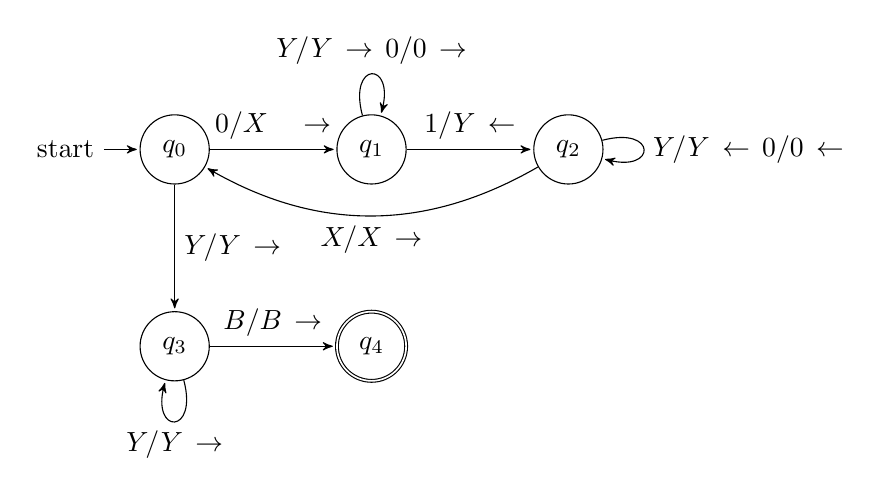
\begin{tikzpicture}[>=stealth',shorten >=1pt,auto,node 
distance=2.5cm]
\node[initial,state]   (q_0)                {$q_0$};
\node[state]           (q_1) [right of=q_0] {$q_1$};
\node[state]           (q_2) [right of=q_1] {$q_2$};
\node[state]           (q_3) [below of=q_0] {$q_3$};
\node[state,accepting] (q_4) [right of=q_3] {$q_4$};
\path[->] (q_0) edge              node {$0/X \quad \rightarrow$} (q_1);
\path[->] (q_1) edge [loop above] node {$Y/Y \, \rightarrow \, 0/0 \, \rightarrow$} (q_1);
\path[->] (q_1) edge              node {$1/Y \, \leftarrow$}     (q_2);
\path[->] (q_2) edge [loop right] node {$Y/Y \, \leftarrow \, 0/0 \, \leftarrow$} (q_2);
\path[->] (q_2) edge [bend left]  node {$X/X \, \rightarrow$}    (q_0);
\path[->] (q_0) edge              node {$Y/Y \, \rightarrow$}    (q_3);
\path[->] (q_3) edge [loop below] node {$Y/Y \, \rightarrow$}    (q_3);
\path[->] (q_3) edge              node {$B/B \, \rightarrow$}    (q_4);
\end{tikzpicture}

Transition diagram for a TM that accepts strings of the form $0^n1^n$

\subsection*{The Language of a Turing Machine}
The input string is placed on the tape, and the tape head begins at the
leftmost input symbol. If the TM eventually enters an accepting state, then
the input is accepted, and otherwise not.

More formally, let $M = (Q,\Sigma,\Gamma,\delta,q_0,B,F)$ be a Turing 
machine. Then $L(M)$ is the set of strings $w$ in $\Sigma^*$ such that 
$q_0w\overset{*}{\vdash} \alpha{p}\beta$ for some state $p$ in $F$ and any
tape strings $\alpha$ and $\beta$.

The set of languages we can accept using a Turing machine is often called 
the \emph{recursively enumerable languages} or RE languages. The term 
``recursively enumberable'' comes from computational formalisms that 
predate the Turing machine but that define the same class of languages or 
arithmetic functions.

\subsection*{Turing Machines and Halting}
There is another notion of ``acceptance'' that is commonly used for Turing
machines: acceptance by halting. We say a TM \emph{halts} if it enters a 
state $q$, scanning a tape symbol $X$, and there is no move in this 
situation; i.e., $\delta(q,X)$ is undefined.

Without changing the language accepted, we can make $\delta(q,X)$ undefined
whether $q$ is an accepting state. In general, without otherwise stating 
so:
\begin{itemize}
\item We assume that a TM always halts when it is in an accepting 
state.
\end{itemize}

Unfortunately, it is not always possible to require that a TM halts even if 
it does not accepts. Those languages with Turing machines that do halt 
eventually, regardless of whether or not they accept, are called 
\emph{recursive}. Turing machines that always halt, regardless of whether 
or not they accept, are a good model of an ``algorithm.'' If an algorithm 
to solve a given problem exists, then we say the problem is ``decidable,''
so TM's that always halt figure importantly into decidability theory.

\subsubsection*{Notaional Conventions for Turing Machines}
The symbols we normally use for Turing machines resemble those for the 
other kinds of automata we have seen.
\begin{enumerate}
\item Lower-case letters at the beginning of the alphabet stand for 
input symbols
\item Capital letters, typically near the end of the alphabet, are 
used for tape symbols that may or may not be input symbols. However, 
$B$ is generally used for the blank symbol.
\item Lower-case letters near the end of the alphabet are strings of 
input symbols.
\item Greek letters are strings of tape symbols
\item Letters such as $q$, $p$, and nearby letters are states.
\end{enumerate}

\section*{Programming Techniques for Turing Machines} 
Turing machines can perform a sort of calculations on other Turing machines. 
This ``introspective'' ability of Turing machines enables us to prove 
problems undecidable.

\subsection*{Storage in the State}
We can use the finite control not only to represent a position in the 
``program'' of the Turing machine, but to hold a finite amount of data. 
Suppose we have a Turing machine that has a finite control consisting of 
not only a ``control'' state $q$, but three data elements $A$, $B$, and 
$C$. The technique requires no extension to the TM model; we merely think 
of the state as a tuple: $\lbrack{}q,A,B,C\rbrack$.

\subsection*{Multiple Tracks}
Another useful ``trick'' is to think of the tape of a Turing machine as 
composed of several tracks. Each track can hold one symbol, and the tape 
alphabet of the TM consists of tuples, with one component for each ``track''.

\subsection*{Subroutines}
A Turing-machine subroutine is a set of states that perform some useful 
process. This set of states includes a start state and another state that 
temporarily has no moves, and that serves as the ``return'' state to pass 
control to whatever other set of states called the subroutine.

\section*{Extensions to the Basic Turing Machine}
\subsection*{Multitape Turing Machines}
A multitape TM has a finite control (state), and some finite number of tapes. 
Each tape is divided into cells, and each cell can hold any symbol of the 
finite tape alphabet. The set of tape symbols includes a blank, and has a 
subset called the input symbols, of which the blank is not a member. The set 
of states includes an initial state and some accepting states. Initially:
\begin{enumerate}
\item The input, a finite sequence of input symbols, is placed on the 
first tape.
\item All other cells of all the tapes hold the blank.
\item The finite control is in the initial state.
\item The head of the first tape is at the left end of the input.
\item All other tape heads are at some arbitrary cell. Since tapes other 
than the first tape are completely blank, it does not matter where the 
head is placed initially; all cells of these tapes ``look'' the same.
\end{enumerate}
A move of the multitape TM depends on the state and teh symbol scanned by each 
of the tape heads. In one move, the multitape TM does the following:
\begin{enumerate}
\item The control enters a new state, which could be the same as the 
previous state.
\item One each tape, a new tape symbols is written on the cell scanned. 
Any of these symbols may be the same as the symbol previously there.
\item Each of the tape heads makes a move, which can be either left, 
right, or stationary. The heads move independently, so different heads may 
move in different directions, and some may not move at all.
\end{enumerate}

\end{document}